\let\negmedspace\undefined
\let\negthickspace\undefined
\documentclass[journal]{IEEEtran}
\usepackage[a4paper, margin=10mm, onecolumn]{geometry}
%\usepackage{lmodern} % Ensure lmodern is loaded for pdflatex
\usepackage{tfrupee} % Include tfrupee package

\setlength{\headheight}{1cm} % Set the height of the header box
\setlength{\headsep}{0mm}  % Set the distance between the header box and the top of the text

\usepackage{gvv-book}
\usepackage{gvv}
\usepackage{cite}
\usepackage{amsmath,amssymb,amsfonts,amsthm}
\usepackage{algorithmic}
\usepackage{graphicx}
\usepackage{float}
\usepackage{textcomp}
\usepackage{xcolor}
\usepackage{txfonts}
\usepackage{listings}
\usepackage{enumitem}
\usepackage{mathtools}
\usepackage{gensymb}
\usepackage{comment}
\usepackage[breaklinks=true]{hyperref}
\usepackage{tkz-euclide} 
\usepackage{listings}
% \usepackage{gvv}                                        
\def\inputGnumericTable{}                                 
\usepackage[latin1]{inputenc}                                
\usepackage{color}                                            
\usepackage{array}                                            
\usepackage{longtable}                                       
\usepackage{calc}                                             
\usepackage{multirow}                                         
\usepackage{hhline}                                           
\usepackage{ifthen}                                           
\usepackage{lscape}
\usepackage{tikz}
\usetikzlibrary{patterns}
\usepackage{multicol}
\begin{document}

\bibliographystyle{IEEEtran}
\vspace{3cm}

\title{GATE-03}
\author{ee25btech11063-vejith}


\maketitle
% \maketitle
% \newpage
% \bigskip
{\let\newpage\relax\maketitle}

\renewcommand{\thefigure}{\theenumi}
\renewcommand{\thetable}{\theenumi}
\setlength{\intextsep}{10pt} % Space between text and floats


\begin{enumerate}
    \item "When she fell down the \underline{\hspace{2cm}} she received many \underline{\hspace{2cm}} but little help." 
    The words that best fill the blanks in the above sentence are
    
    \hfill{\brak{\text{GATE GG 2018}}}
    \begin{enumerate}
        \begin{multicols}{2}
            \item stairs, stares
            \item stairs, stairs
            \item stares, stairs
            \item stares, stares
        \end{multicols}
    \end{enumerate}

    \item "In spite of being warned repeatedly, he failed to correct his \underline{\hspace{2cm}} behaviour."
    The word that best fills the blank in the above sentence is
    
    \hfill{\brak{\text{GATE GG 2018}}}
    \begin{enumerate}
        \begin{multicols}{4}
            \item rational
            \item reasonable
            \item errant
            \item good
        \end{multicols}
    \end{enumerate}

    \item For $0 \le x \le 2\pi$, $\sin x$ and $\cos x$ are both decreasing functions in the interval
    
    \hfill{\brak{\text{GATE GG 2018}}}
    \begin{enumerate}
        \begin{multicols}{4}
            \item $\brak{0,\frac{\pi}{2}}$
            \item $\brak{\frac{\pi}{2},\pi}$
            \item $\brak{\pi,\frac{3\pi}{2}}$
            \item $\brak{\frac{3\pi}{2},2\pi}$
        \end{multicols}
    \end{enumerate}

    \item The area of an equilateral triangle is $\sqrt{3}$. What is the perimeter of the triangle?
    
    \hfill{\brak{\text{GATE GG 2018}}}
    \begin{enumerate}
        \begin{multicols}{4}
            \item $2$
            \item $4$
            \item $6$
            \item $8$
        \end{multicols}
    \end{enumerate}

    \item Arrange the following three-dimensional objects in the descending order of their volumes:
    \begin{itemize}
        \item \brak{i} A cuboid with dimensions $10$ cm, $8$ cm and $6$ cm
        \item \brak{ii} A cube of side $8$ cm
        \item \brak{iii} A cylinder with base radius $7$ cm and height $7$ cm
        \item \brak{iv} A sphere of radius $7$ cm
    \end{itemize}
    
    \hfill{\brak{\text{GATE GG 2018}}}
    \begin{enumerate}
        \begin{multicols}{2}
            \item \brak{i}, \brak{ii}, \brak{iii}, \brak{iv}
            \item \brak{ii}, \brak{i}, \brak{iv}, \brak{iii}
            \item \brak{iii}, \brak{ii}, \brak{i}, \brak{iv}
            \item \brak{iv}, \brak{iii}, \brak{ii}, \brak{i}
        \end{multicols}
    \end{enumerate}

    \item An automobile travels from city A to city B and returns to city A by the same route. The speed of the vehicle during the onward and return journeys were constant at $60$ km/h and $90$ km/h respectively. What is the average speed in km/h for the entire journey?
    
    \hfill{\brak{\text{GATE GG 2018}}}
    \begin{enumerate}
        \begin{multicols}{4}
            \item $72$
            \item $73$
            \item $74$
            \item $75$
        \end{multicols}
    \end{enumerate}

    \item A set of $4$ parallel lines intersect with another set of $5$ parallel lines. How many parallelograms are formed?
    
    \hfill{\brak{\text{GATE GG 2018}}}
    \begin{enumerate}
        \begin{multicols}{4}
            \item $20$
            \item $48$
            \item $60$
            \item $72$
        \end{multicols}
    \end{enumerate}
    
    \item To pass a test, a candidate needs to answer at least $2$ out of $3$ questions correctly. A total of $6,30,000$ candidates appeared for the test. Question A was correctly answered by $3,30,000$ candidates. Question B was answered correctly by $2,50,000$ candidates. Question C was answered correctly by $2,60,000$ candidates. Both questions A and B were answered correctly by $1,00,000$ candidates. Both questions B and C were answered correctly by $90,000$ candidates. Both questions A and C were answered correctly by $80,000$ candidates. If the number of students answering all questions correctly is the same as the number answering none, how many candidates failed to clear the test?
    
    \hfill{\brak{\text{GATE GG 2018}}}
    \begin{enumerate}
        \begin{multicols}{4}
            \item $30,000$
            \item $2,70,000$
            \item $3,90,000$
            \item $4,20,000$
        \end{multicols}
    \end{enumerate}

    \item If $x^{2}+x-1=0$ what is the value of $x^{4}+\frac{1}{x^{4}}$?
    
    \hfill{\brak{\text{GATE GG 2018}}}
    \begin{enumerate}
        \begin{multicols}{4}
            \item $1$
            \item $5$
            \item $7$
            \item $9$
        \end{multicols}
    \end{enumerate}
    
    \item In a detailed study of annual crow births in India, it was found that there was relatively no growth during the period $2002$ to $2004$ and a sudden spike from $2004$ to $2005$. In another unrelated study, it was found that the revenue from cracker sales in India which remained fairly flat from $2002$ to $2004$, saw a sudden spike in $2005$ before declining again in $2006$. The solid line in the graph below refers to annual sale of crackers and the dashed line refers to the annual crow births in India. Choose the most appropriate inference from the above data.
    \begin{figure}[H]
        \centering
        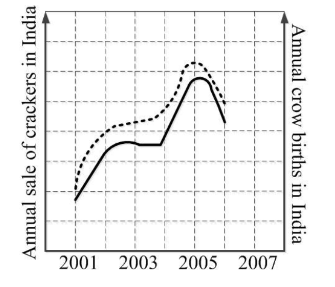
\includegraphics[width=0.5\columnwidth]{figs/01.png}
        \caption*{}
        \label{fig:q10}
    \end{figure}
    
    \hfill{\brak{\text{GATE GG 2018}}}
    \begin{enumerate}
        \item There is a strong correlation between crow birth and cracker sales.
        \item Cracker usage increases crow birth rate.
        \item If cracker sale declines, crow birth will decline.
        \item Increased birth rate of crows will cause an increase in the sale of crackers.
    \end{enumerate}
\textbf{END OF THE QUESTION PAPER}
\end{enumerate}
\vspace{1cm}
\begin{enumerate}[start=1]
    \item  Which one of the following periods has the longest time duration? 
\hfill(GATE GG 2018)
\begin{multicols}{4}
\begin{enumerate}
\item Ordovician
\item Cretaceous
\item Jurassic
\item Silurian
\end{enumerate}
\end{multicols}

\item  A siliciclastic sedimentary rock consisting predominantly of the same type of gravel-sized clasts is called  
\hfill(GATE GG 2018)
\begin{multicols}{2}
\begin{enumerate}
\item Polymict conglomerate
\item Arkose
\item Oligomict conglomerate
\item Petromict conglomerate
\end{enumerate}
\end{multicols}

\item Brown coal that has high moisture content and commonly retains many of the original wood fragments is called\\
\hspace*{15.7cm}(GATE GG 2018)
\begin{multicols}{2}
\begin{enumerate}
\item Anthracite
\item Bituminous coal
\item Lignite
\item Peat
\end{enumerate}
\end{multicols} 

\item The speed of revolution of the Earth around the Sun is  

\hfill(GATE GG 2018)
\begin{enumerate}
\item maximum at Perihelion
\item minimum at Perihelion
\item maximum at Aphelion
\item equal at Aphelion and Perihelion
\end{enumerate}

\item The geometrical factor for the following electrode configuration is  

\hfill(GATE GG 2018)
 \begin{figure}[H]
        \centering
        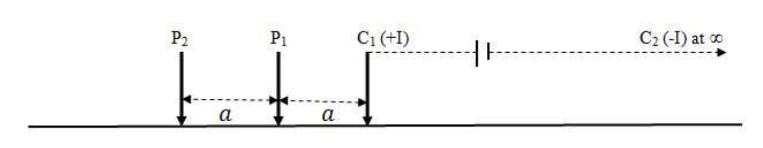
\includegraphics[width=0.5\columnwidth]{figs/02.png}
        \caption*{}
        \label{fig:q10}
    \end{figure}
    \begin{multicols}{4}
\begin{enumerate}
\item $\pi a$
\item $2\pi a$
\item $3\pi a$
\item $4\pi a$
\end{enumerate}
\end{multicols}

\item Which one of the following geophysical methods uses the physical property Dielectric Constant ?  

\hfill(GATE GG 2018)
\begin{multicols}{2}
\begin{enumerate}
\item Gravity
\item Ground Penetrating Radar
\item Seismic
\item Self-Potential
\end{enumerate}
\end{multicols}

\item  Pascal second is a unit of  

\hfill(GATE GG 2018)
\begin{multicols}{2}
\begin{enumerate}
\item seepage force
\item dynamic viscosity
\item kinematic viscosity
\item permeability
\end{enumerate}
\end{multicols}

\item  Which one of the following statements is CORRECT?  

\hfill(GATE GG 2018)
\begin{enumerate}
\item Strength of a rock decreases with increase in confining pressure
\item Strength of a rock increases with increase in temperature
\item Strength of a rock increases with increase in strain rate
\item Strength of a rock increases with increase in pore water pressure
\end{enumerate}

\item The geomorphic feature horns  are formed by 

\hfill(GATE GG 2018)
\begin{multicols}{2}
\begin{enumerate}
\item wind erosion
\item river erosion
\item wind deposition
\item glacial erosion
\end{enumerate}
\end{multicols}

\item A melanocratic porphyritic rock containing phenocrysts of biotite, with feldspar restricted to the groundmass, is called  

\hfill(GATE GG 2018)
\begin{multicols}{4}
\begin{enumerate}
\item trachyte
\item dacite
\item andesite
\item lamprophyre
\end{enumerate}
\end{multicols}

\item The supercontinent that existed in the late Mesoproterozoic to early Neoproterozoic time was  
\hfill(GATE GG 2018)
\begin{multicols}{4}
\begin{enumerate}
\item Kenorland
\item Columbia
\item Rodinia
\item Pangaea
\end{enumerate}
\end{multicols}

\item The figure below shows the triple junction between three plates A, B and C. The boundary between the plates A and B is a ridge with a half-spreading rate of $4$ cm/year. The A-C and B-C boundaries are collinear and orthogonal to the A-B ridge. The A-C boundary is a dextral transform fault with a relative velocity of $6$ cm/year. The boundary between plates B and C is: 
\hfill(GATE GG 2018)
\begin{figure}[H]
        \centering
	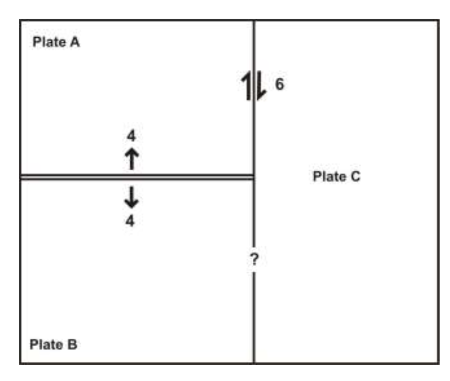
\includegraphics[width=0.5\columnwidth]{figs/03.png}
        \caption*{}
        \label{fig:q10}
    \end{figure}
\begin{enumerate}
\item dextral transform fault with a relative velocity of $10$ cm/year
\item dextral transform fault with a relative velocity of $2$ cm/year
\item sinistral transform fault with a relative velocity of $2$ cm/year
\item sinistral transform fault with a relative velocity of $6$ cm/year
\end{enumerate}

\item A rock follows Mohr-Coulomb failure criterion. Which one of the Mohr-Coulomb failure envelopes allows failure of the rock under stress state Y, but not under stress state X?  
\hfill(GATE GG 2018)
\begin{figure}[H]
        \centering
        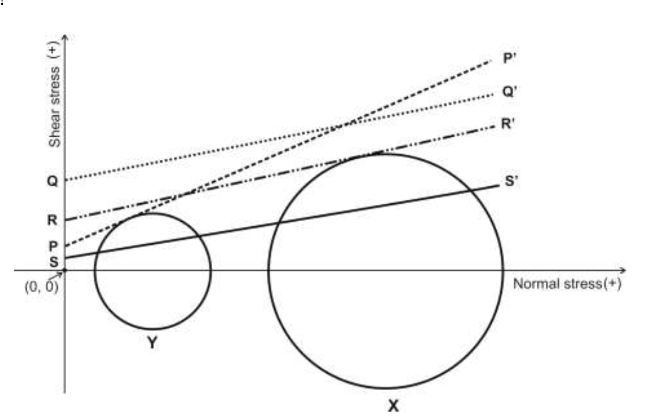
\includegraphics[width=0.5\columnwidth]{figs/04.png}
        \caption*{}
        \label{fig:q10}
    \end{figure}
\begin{multicols}{4}
\begin{enumerate}
\item PP$'$
\item QQ$'$
\item RR$'$
\item SS$'$
\end{enumerate}
\end{multicols}

\item The maximum and the minimum principal stresses are denoted by $\sigma_1$ and $\sigma_3$, respectively. 
The differential stress can have an absolute value greater than $\sigma_1$ when  
\hfill(GATE GG 2018)
\begin{enumerate}
\item $\sigma_1$ and $\sigma_3$ are both compressive
\item $\sigma_1$ is compressive and $\sigma_3$ is tensile
\item $\sigma_1$ and $\sigma_3$ are equal
\item $\sigma_1$ and $\sigma_3$ are both tensile
\end{enumerate}

\item The geoid can be best defined as  
\hfill(GATE GG 2018)
\begin{enumerate}
\item an oblate spheroid that best approximates the shape of the earth
\item a surface over which the value of gravity is constant
\item the physical surface of the earth
\item an equipotential surface of gravity of the earth
\end{enumerate}

\item For a layered isotropic medium with a flat horizontal free surface, match the wave types listed in Group-I with their corresponding polarizations in Group-II.
\hfill(GATE GG 2018)
\begin{tabular}{ l l }
\textbf{Group I} & \textbf{Group Il}\\
(P) P-waves & particle motion is transverse to the direction of wave propagation\\
(Q) Q-waves & particle motion is transverse to the direction of wave propagation and confined to the horizontal plane\\
(R) Rayleigh waves & particle motion is parallel  to the direction of wave propagation\\
(S) Love waves & particle motion is elliptical
\end{tabular}
\begin{multicols}{2}
\begin{enumerate}
\item P-1; Q-3; R-4; S-2
\item P-3; Q-1; R-4; S-2
\item P-3; Q-1; R-2; S-4
\item P-2; Q-3; R-1; S-4
\end{enumerate}
\end{multicols}

\item A $'\text{gentle}'$ fold with an interlimb angle equal to $160^\degree$ appears tight (apparent interlimb angle equal to $20^\degree$) in horizontal section. According to the plunge of the fold axis, it can also be classified as
\hfill(GATE GG 2018)
\begin{multicols}{2}
\begin{enumerate}
\item horizontal fold
\item gently plunging fold
\item steeply plunging fold
\item vertical fold
\end{enumerate}
\end{multicols}

\item The unit of shear modulus (rigidity modulus) is  
\hfill(GATE GG 2018)
\begin{multicols}{2}
\begin{enumerate}
\item kg m$^{-1}$s$^{-2}$
\item m$^2$ s$^{-2}$
\item kg m$^{-2}$ s$^{-2}$
\item m$^{-1}$
\end{enumerate}
\end{multicols}

\item With increasing activity of silica, the CORRECT order of appearance of minerals in a 
weathering environment with constant ratio of activities of K$^+$ and H$^+$ is  
\hfill(GATE GG 2018)
\begin{enumerate}
\item gibbsite $\to$ kaolinite $\to$ pyrophyllite
\item gibbsite $\to$ pyrophyllite $\to$ kaolinite
\item kaolinite $\to$ gibbsite $\to$ pyrophyllite
\item pyrophyllite $\to$ gibbsite $\to$ kaolinite
\end{enumerate}

\item Match the items listed in Group-I with those in Group-II.\\
\hspace*{15.7cm}(GATE GG 2018)\\
\begin{tabular}{ l l }
\textbf{Group I} & \textbf{Group Il}\\
(P) Mica & 1.Beldih\\
(Q) Uranium & 2.Koderma\\
(R) Phosphate & 3.Agucha\\
(S) Zinc & 4.Gochi
\end{tabular}
\begin{multicols}{2}
\begin{enumerate}
\item P-2, Q-3, R-4, S-1
\item P-2, Q-4, R-1, S-3
\item P-4, Q-2, R-3, S-1
\item P-3, Q-1, R-4, S-2
\end{enumerate}
\end{multicols}

\item Which one of the following corrections is always added during reduction of the observed gravity data?  
\hfill(GATE GG 2018)
\begin{multicols}{4}
\begin{enumerate}
\item Latitude
\item Free-air
\item Bouguer
\item Terrain
\end{enumerate}
\end{multicols}

\item The magnitudes of the total geomagnetic field at the equator and pole are denoted by $B_E$ and $B_P$, respectively. Which one of the following is TRUE?  
\hfill(GATE GG 2018)
\begin{multicols}{2}
\begin{enumerate}
\item $B_P \approx 4 B_E$
\item $B_P \approx 2 B_E$
\item $B_P \approx B_E$
\item $B_P \approx \tfrac{1}{2} B_E$
\end{enumerate}
\end{multicols}

\item Assume a flat earth with crustal thickness of 35 km and average crustal and upper mantle P-wave velocities of $6.4$ km/s and $8.1$ km/s, respectively. The minimum distance from the epicenter of a near-surface earthquake at which P$_n$-waves are observed is  \makebox[2cm]{\hrulefill} km.
\hfill(GATE GG 2018)
\vspace{0.7cm}
\item Given that the velocity of P-waves in a sandstone matrix is $5600$ m/s and that in oil is $1200$ m/s, the velocity of P-wave propagation in oil-saturated sandstone with $30$\% porosity is \makebox[2cm]{\hrulefill} m/s. \brak{\text{Use Wyllie time average equation.}}
\hspace*{15.7cm}(GATE GG 2018)
\vspace{1cm}

  \item If the total porosity of a soil is $20$\%, its void ratio \brak{\%} is \makebox[2cm]{\hrulefill}
  \hfill(GATE GG 2018)\\

\textbf{PART B(SECTION 1):FOR GEOLOGY CANDIDATES ONLY}
\vspace{0.7cm}
  \item Which one of the following Himalayan lithounits predates India-Eurasia collision?  
  \hfill(GATE GG 2018)
\begin{multicols}{2}
\begin{enumerate}
\item Kasauli sandstone
\item Rangit Pebble Slate
\item Annapurna granite
\item Lower Karewa sandstone
\end{enumerate}
\end{multicols}

\item Which one of the following ore minerals shows internal reflection? 
\hfill(GATE GG 2018)
\begin{multicols}{4}
\begin{enumerate}
\item Orpiment
\item Magnetite
\item Pyrite
\item Molybdenite
\end{enumerate}
\end{multicols}

\item Which one is CORRECT for the following equilibrium reaction between quartz and magnetite:\\ 
$\text{Si}^{16}\text{O}^{16}\text{O} + \text{Fe}_3^{16}\text{O}_3^{18}\text{O} = \text{Si}^{16}\text{O}^{18}\text{O} + \text{Fe}_3^{16}\text{O}_4$ ?  
\hfill(GATE GG 2018)
\begin{enumerate}
\item $1000 \ln \alpha = \Delta_{\text{qtz-mag}},\ \alpha = K^{1/n}$ (K equilibrium constant at specified T, n constant)
\item $1000 \ln \alpha = \Delta_{\text{qtz-mag}},\ \alpha = K^n$ (K equilibrium constant, n = no. of exchangeable sites)
\item $(\ln \alpha /1000) = \Delta_{\text{qtz-mag}},\ \alpha = K^{1/n}$ (K equilibrium constant, n constant)
\item $1000 \ln \alpha = \Delta_{\text{qtz-mag}},\ \alpha = K^{1/n}$ (K equilibrium constant, n = no. of exchangeable sites)
\end{enumerate}

\item Match the modes of life \brak{\text{Group I}} with the corresponding bivalve genera \brak{\text{Group II}}
\hfill(GATE GG 2018)\\
\begin{tabular}{ l l }
\textbf{Group I} & \textbf{Group Il}\\
(P) Burrowing & 1. (1) Mytilus\\
(Q) Recumbent unattached & 2. Pecten\\
(R) Byssally attached & (3) Mya\\
(S) Swimming & 4. Gryphaea
\end{tabular}
\begin{multicols}{2}
\begin{enumerate}
\item P-4, Q-3, R-2, S-1
\item P-3, Q-4, R-1, S-2
\item P-2, Q-3, R-1, S-4
\item P-3, Q-1, R-4, S-2
\end{enumerate}
\end{multicols}

\item Based on the hypothetical litholog continuous succession of sedimentary rocks , which one statement is CORRECT?  
\begin{figure}[H]
        \centering
        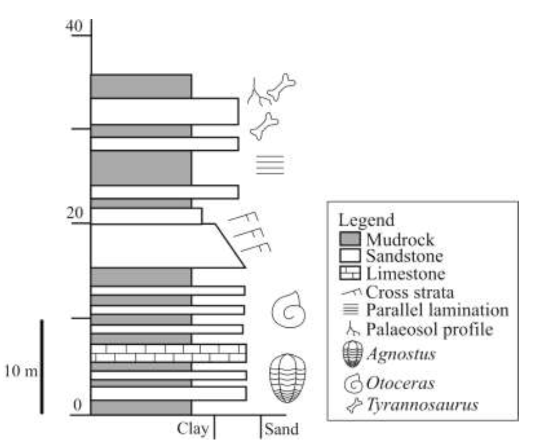
\includegraphics[width=0.5\columnwidth]{figs/05.png}
        \caption*{}
        \label{fig:q10}
    \end{figure}
    \hfill(GATE GG 2018)
\begin{enumerate}
\item Cambrian to Cretaceous, change from marine $\rightarrow$ continental
\item Cambrian to Triassic, change from marine $\rightarrow$ continental
\item Cambrian to Cretaceous, change from continental $\rightarrow$ marine
\item Palaeozoic in age, change from marine $\rightarrow$ continental
\end{enumerate}

\item Which cladogram shows the CORRECT interrelationships among the major groups of vertebrates? 
\begin{figure}[H]
        \centering
        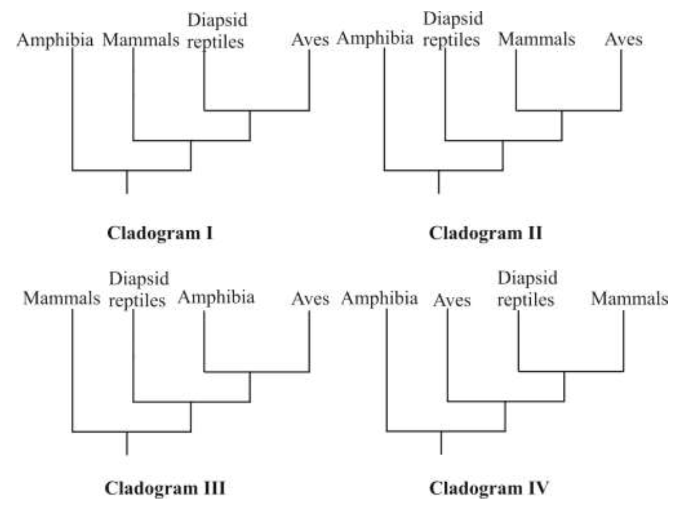
\includegraphics[width=0.5\columnwidth]{figs/06.png}
        \caption*{}
        \label{fig:q10}
    \end{figure}
    \hfill(GATE GG 2018)
\begin{multicols}{4}
\begin{enumerate}
\item Cladogram I
\item Cladogram II
\item Cladogram III
\item Cladogram IV
\end{enumerate}
\end{multicols}

\item Which one of the following stratigraphic successions is in the CORRECT chronological order \brak{\text{older to younger}}?  
\hspace*{15.7cm}(GATE GG 2018)
\begin{enumerate}
\item Rajmahal, Dubrajpur, Barakar
\item Fenestella Shale, Muth Quartzite, Syringothyris Limestone
\item Bagh Bed, Lameta Formation, Deccan Traps
\item Singhbhum Granite, Kolhan Group, Older Metamorphic Gneiss
\end{enumerate}

\item  Match the items in Group I with Group II
\hfill(GATE GG 2018)\\
\begin{tabular}{ l l }
\textbf{Group I} & \textbf{Group Il}\\
(P) Peloids &  (1) Nucleus with irregular laminae\\
 (Q) Ooids &  (2) Micritic grains no structure\\
  (R) Oncoids & (3) Rounded grains thin micrite coating\\
  (S) Cortoids & (4) Spherical grains concentric laminae 
\end{tabular}
\begin{multicols}{2}
\begin{enumerate}
\item P-3, Q-1, R-4, S-2
\item P-2, Q-4, R-1, S-3
\item P-3, Q-4, R-1, S-2
\item P-2, Q-3, R-4, S-1
\end{enumerate}
\end{multicols}

\item Which one of the following is an image rectification technique?  
\hfill(GATE GG 2018)
\begin{enumerate}
\item Histogram equalization
\item Density slicing
\item Histogram normalization
\item Rubbersheeting
\end{enumerate}

\item Match Group I with Group II.
\hfill(GATE GG 2018)\\
\begin{tabular}{ l l }
\textbf{Group I} & \textbf{Group Il}\\
(P) Coefficient of compressibility of soils & (1) Brazilian test\\
(Q) Method of slope stabilization & (2) Overcoring\\
(R) In situ stress determination & (3) Oedometer test\\
(S) Indirect tensile strength of rocks & (4) Shotcreting  
\end{tabular}
\begin{multicols}{2}
\begin{enumerate}
\item P-4, Q-2, R-3, S-1
\item P-1, Q-4, R-2, S-3
\item P-3, Q-2, R-1, S-4
\item P-3, Q-4, R-2, S-1
\end{enumerate}
\end{multicols}

\item Match the items listed in Group I with those listed in Group II.
\hfill(GATE GG 2018)\\
\begin{tabular}{ l l }
\textbf{Group I} & \textbf{Group Il}\\
(P) Crevasse &  (1) River\\
(Q) Yardang &  (2) Groundwater\\
 (R) Mesa & (3) Wind\\
 (S) Stalactite & (4) Glacier
\end{tabular}
\begin{multicols}{2}
\begin{enumerate}
\item P-4, Q-3, R-1, S-2
\item P-3, Q-1, R-4, S-2
\item P-4, Q-2, R-3, S-1
\item P-1, Q-2, R-3, S-4
\end{enumerate}
\end{multicols}

\item In the hypothetical isobaric ternary liquids projection diagram shown, solid phases A, B, C, D and E exist in equilibrium with liquid. The reaction taking place at the isobaric invariant point W is 
\hfill(GATE GG 2018)
\begin{multicols}{2}
\begin{enumerate}
\item Liquid \brak{\text{at W}} $=$ B $+$ D $+$ E
\item Liquid  \brak{\text{at W}} $=$ A $+$ B $+$ D
\item Liquid \brak{\text{at W}} $+$ E $=$ B $+$ D
\item Liquid \brak{\text{at W}} $+$ B $+$ D $=$ E
\end{enumerate}
\end{multicols}

\item Match the optical properties (Group I) with the corresponding mineral (Group II).  
\hfill(GATE GG 2018)\\
\begin{tabular}{ l l }
\textbf{Group I} & \textbf{Group Il}\\
P. Brown colour, very high RI, very high birefringence, biaxial positive & (1) Apatite\\
Q. Colourless, very high RI, low birefringence, uniaxial negative & (2) Rutile\\
R. Deep reddish-brown, very high RI, very high birefringence, uniaxial positive & (3) Zircon\\
S. Colourless, very high RI, very high birefringence, uniaxial positive & (4) Titanite  
\end{tabular}
\begin{multicols}{2}
\begin{enumerate}
\item P-4, Q-1, R-2, S-3
\item P-1, Q-2, R-4, S-3
\item P-3, Q-4, R-1, S-2
\item P-4, Q-1, R-3, S-2
\end{enumerate}
\end{multicols}

\item The reaction  
muscovite $+$ quartz $=$ K-feldspar $+$ sillimanite $+$ water  
\hfill(GATE GG 2018)
\begin{multicols}{2}
\begin{enumerate}
\item takes place within the greenschist facies
\item takes place within the amphibolite facies
\item takes place within the eclogite facies
\item takes place within the granulite facies
\end{enumerate}
\end{multicols}

\item Match the mineral assemblages (Group I) with rock types (Group II).
\hfill(GATE GG 2018)\\
\begin{tabular}{ l l }
\textbf{Group I} & \textbf{Group Il}\\
(P) Diopside-tremolite-forsterite & 1. Pelite (low P, high T)\\
(Q) Talc-phengite-kyanite &  (2) Metabasite (low P, high T)\\
 (R) Hornblende-cummingtonite-plagioclase & (3) Calc-silicate (moderate P, T)\\
 (S) Andalusite-cordierite-biotite & (4) Pelite (high P, low T)  
\end{tabular}
\begin{multicols}{2}
\begin{enumerate}
\item P-3, Q-4, R-1, S-2
\item P-1, Q-2, R-4, S-3
\item P-3, Q-4, R-2, S-1
\item P-1, Q-2, R-3, S-4
\end{enumerate}
\end{multicols}

\item The figure shows the initial stages of development of a thrust fault \brak{\text{FF}} with ramp and flat geometry, moving east to  west. With respect to synform and antiform in Stage 2, the next increment of movement will:  
\hfill(GATE GG 2018)
\begin{figure}[H]
        \centering
        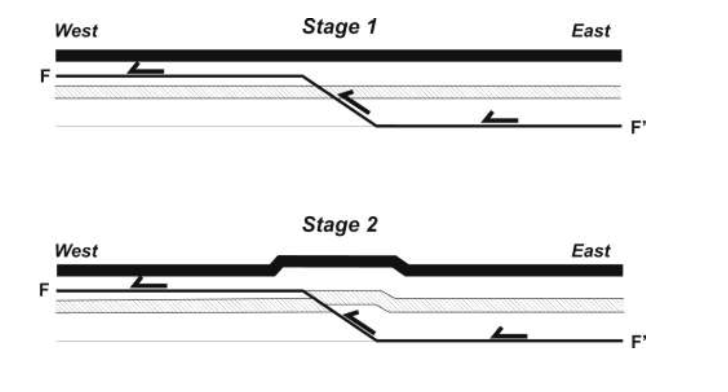
\includegraphics[width=0.6\columnwidth]{figs/07.png}
        \caption*{}
        \label{fig:q10}
    \end{figure}
\begin{enumerate}
\item Both synform and antiform move westward
\item Synform stays, antiform amplitude grows
\item Both synform and antiform amplitudes grow
\item Geometry remains unchanged
\end{enumerate}

\item Which one of the following is the CORRECT chronological sequence for Iron formations?  
\hfill(GATE GG 2018)
\begin{enumerate}
\item Algoma type $>$ Superior type $>$ Rapitan type $>$ Minette type
\item Superior type $>$ Algoma type $>$ Rapitan type $>$ Minette type
\item Rapitan type $>$ Minette type $>$ Algoma type $>$ Superior type
\item Algoma type $>$ Minette type $>$ Superior type $>$ Rapitan type
\end{enumerate}

\item Assertion \brak{\text{a}}: High-temperature, low-pressure metamorphism occurs on the over-riding plate near convergent plate margins.  
Reason \brak{\text{r}}: Partial melting in the mantle wedge generates magmas that rise to form the arc. 
\hfill(GATE GG 2018)
\begin{enumerate}
\item (a) true, (r) false
\item (a) false, (r) true
\item Both true and (r) is correct reason
\item Both true but (r) not the correct reason
\end{enumerate}

\item Two coeval aqueous biphase fluid inclusions X \brak{\text{liquid-rich}} and Y \brak{\text{vapour-rich}} occur in the same grain. Which indicates boiling?  
\hfill(GATE GG 2018)
\begin{enumerate}
\item X homogenizes to  liquid and Y homogenizes to a vapour at different temperatures.
\item Both homogenizes to  liquid at same temperatures.
\item Both homogenizes to  liquid at same temperatures.
\item X homogenizes to  liquid and Y homogenizes to a vapour at same  temperatures
\end{enumerate}
\vspace{0.7cm}
\item During bench blasting in a quarry, $50$ kg of explosive with yield of $5$ MJ/kg is required to break $100$ m$^3$ of marble. The energy expended per unit volume of marble in MN/m$^2$ is \makebox[2cm]{\hrulefill}
\hfill(GATE GG 2018)
\vspace{0.5cm}
\item The stretching lineation on the axial plane \brak{\text{S2}} of a reclined fold on the S1 foliation makes an angle of 30$\degree$ with the S1/S2 intersection lineation.  The rake of the stretching lineation on the axial plane in degrees is \makebox[2cm]{\hrulefill}
\hfill(GATE GG 2018)
\vspace{0.5cm}

\item A basaltic magma has an initial nickel concentration of 300 ppm. Olivine crystallizes from this magma by equilibrium crystallization \brak{\text{Case I}}or fractional crystallization \brak{\text{Case II}}. Then, the absolute value of the difference between the nickel concentrations of the liquids remaining after 25\% crystallization in these two cases is \makebox[2cm]{\hrulefill}.  
\brak{\text{Use $K_{D,Ni}{\text{olivine/melt}} = 10$}}.
\hspace*{15.7cm}(GATE GG 2018)
\vspace{0.5cm}

\item The difference in the number of faces in forms \cbrak{hkl} and \cbrak{111} in the holosymmetric class of the isometric system is \makebox[2cm]{\hrulefill}
\hspace*{15.7cm}(GATE GG 2018)
\vspace{0.5cm}
\item An inclined cylindrical confined aquifer has coefficient of permeability of $40$ m/day.  The horizontal distance between two vertical wells penetrating the aquifer is $800$ m.  The water surface elevations in the wells are $50$ m and $45$ m above a common horizontal datum.  The absolute value of Darcy flux through the aquifer is \makebox[2cm]{\hrulefill} m/day.
\hfill(GATE GG 2018)
\vspace{0.5cm}

\item The mass and volume of a natural soil sample are $2.1$ kg and $1\times 10^{-3}$ m$^3$, respectively.  When fully dried, the mass of the soil sample becomes $2$ kg without any change in volume.  Assuming the specific gravity of soil particles to be $2.5$, and water density of 1000 kg/m$^3$,  the degree of saturation of the natural soil sample is \makebox[2cm]{\hrulefill}\% .
\hfill(GATE GG 2018)
\vspace{0.5cm}

\item For a granitic rock mass, joint set number \brak{\text{Jn}} = $9$, joint water reduction factor \brak{\text{Jw }}$= 1$,  joint alteration number \brak{\text{Ja}} $= 1$, stress reduction factor \brak{\text{SRF}} $= 1$, rock quality designation \brak{\%} $= 84$,  and joint roughness number \brak{\textbf{Jr}} $= 3$.  The Q-value as per Barton$'$s Q-system of rock mass classification \brak{\text{1974}} is 
\hfill(GATE GG 2018)
\vspace{0.5cm}

\item A sun synchronous satellite is at an altitude of $300$ km and the spectrometer makes an  angular coverage angle of $12\degree$. The Swath \brak{\text{ GFOV}} of the satellite is \makebox[2cm]{\hrulefill} km.
\hfill(GATE GG 2018)
\vspace{0.5cm}
\item The stability field boundary between two minerals A and B is linear with a positive slope in P-T space. The molar entropy of A and B are $85.5$ and $92.5$ J K$^{-1}$ respectively, and their respective molar volumes are $35.5$ and $38.2$ cc.  
The slope of the phase boundary in P-T space is \makebox[2cm]{\hrulefill} bar K$^{-1}$.
\hfill(GATE GG 2018)
\vspace{0.5cm}

\item Five moles of gas A (volume $V_1$) and three moles of gas B (volume $V_2$) were kept in two separate containers. These two gases are completely transferred to a new container of volume $V$. Assuming isothermal conditions and that the work done is only mechanical,  the entropy change of the system is \makebox[2cm]{\hrulefill} J K$^{-1}$. (R = 8.3 J K$^{-1}$ mol$^{-1}$)
\hfill(GATE GG 2018)
\vspace{0.5cm}

\item The value of Eh corresponding to the upper limit of natural surface aqueous environment at pH = $8.0$ is \makebox[2cm]{\hrulefill}  V.
\hspace*{15.7cm}(GATE GG 2018)
\textbf{PART B(SECTION 2):FOR GEOPHYSICS CANDIDATES ONLY}
\vspace{1cm}
\item The maximum number of linearly independent rows of an $m \times n$ matrix $G$ where $m>n$ is
\hfill(GATE GG 2018)
\begin{multicols}{2}
\begin{enumerate}
\item $m$
\item $n$
\item $m-n$
\item 0
\end{enumerate}
\end{multicols}

\item The impulse response of the Kirchhoff pre-stack time migration operator for non-zero offsets in a homogeneous and isotropic medium is
\hfill(GATE GG 2018)
\begin{multicols}{2}
\begin{enumerate}
\item a circle
\item a parabola
\item a hyperbola
\item an ellipse
\end{enumerate}
\end{multicols}

\item A solution to the eikonal equation $|\nabla \tau| = \tfrac{1}{v_0}$ for a homogeneous and isotropic medium in Cartesian coordinates is\\
\hspace*{15.7cm}(GATE GG 2018)
\begin{multicols}{2}
\begin{enumerate}
\item $\tau = \dfrac{\sqrt{x^2+y^2+z^2}}{v_0}$
\item $\tau = \dfrac{1}{v_0}$
\item $\tau = \dfrac{x+y+z}{v_0}$
\item $\tau = \dfrac{xyz}{v_0}$
\end{enumerate}
\end{multicols}

\item The forward Fourier transform is $F(\omega) = \int_{-\infty}^{\infty} f(t) e^{-i\omega t} dt$  
and the inverse Fourier transform is $f(t) = \int_{-\infty}^{\infty}F(\omega)e^{i\omega t}d\omega$.  
Then, the forward Fourier transform of $F(\omega)=e^{-2i\omega}$ is
\hfill(GATE GG 2018)
\begin{multicols}{4}
\begin{enumerate}
\item $2\delta(t)$
\item $\delta(2t)$
\item $\delta(t+2)$
\item $\delta(t-2)$
\end{enumerate}
\end{multicols}

\item Which one of the following rock types has the highest bulk magnetic susceptibility value?
\hfill(GATE GG 2018)
\begin{enumerate}
\item Gabbro
\item Marble
\item Orthoquartzite
\item Limestone
\end{enumerate}

\item Figure 1 is a schematic of seismic events in t-x\brak{\text{time-offset}} domain and Figure 2 is the corresponding transformation to f-kx \brak{\text{frequency-horizontal wavenumber}} domain. Match events in Figure 1 with those in Figure 2.
\hfill(GATE GG 2018)
\begin{figure}[H]
        \centering
        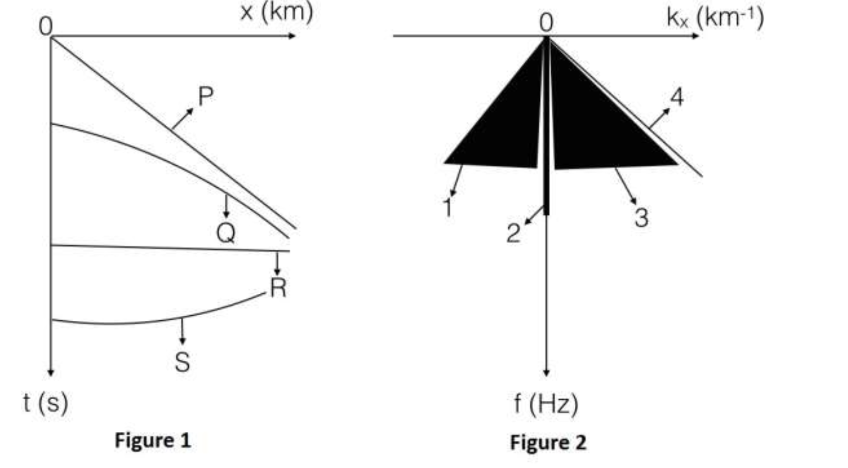
\includegraphics[width=0.5\columnwidth]{figs/08.png}
        \caption*{}
        \label{fig:q10}
    \end{figure}
    \begin{multicols}{2}
\begin{enumerate}
\item P-1; Q-2; R-3; S-4
\item P-1; Q-3; R-2; S-4
\item P-4; Q-3; R-2; S-1
\item P-4; Q-2; R-3; S-1
\end{enumerate}
\end{multicols}

\item Across the Gutenberg discontinuity \brak{\text{from mantle to outer core}} there is a change of bulk modulus and density. Which one of the following is CORRECT?
\hfill(GATE GG 2018)
\begin{multicols}{2}
\begin{enumerate}
\item Both bulk modulus and density increase
\item Both bulk modulus and density decrease
\item Bulk modulus decreases and density increases
\item Bulk modulus increases and density decreases
\end{enumerate}
\end{multicols}

% Q63
\item Multi-electrode resistivity survey is carried out with $10$ equispaced electrodes. \brak{\text{denoted by arrows in the figure below}} Considering the mid-point of the $4$-electrode array as the point of observation laterally,  
identify the CORRECT configuration.
\hspace*{15.7cm}(GATE GG 2018)
\begin{figure}[H]
        \centering
        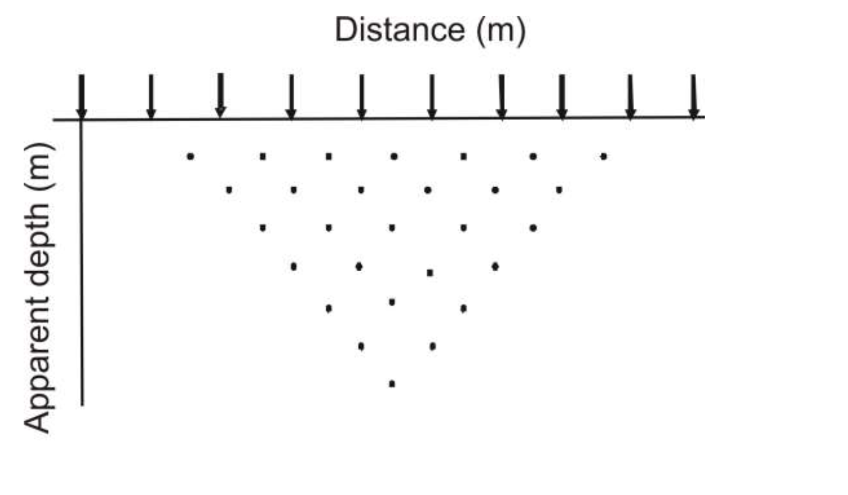
\includegraphics[width=0.5\columnwidth]{figs/09.png}
        \caption*{}
        \label{fig:q10}
    \end{figure}
\begin{multicols}{2}
\begin{enumerate}
\item Multi-electrode Wenner array
\item Multi-electrode Axial Dipole-dipole array
\item Multi-electrode Wenner-Schlumberger array
\item Multi-electrode Axial Pole-dipole array
\end{enumerate}
\end{multicols}

\item Match the electromagnetic methods in Group I with the corresponding quantities measured in Group II.  .
\hfill(GATE GG 2018)\\
\begin{tabular}{ l l }
\textbf{Group I} & \textbf{Group Il}\\
(P) AFMAG method & 1.Decay of secondary field\\
Q) Time domain EM & 2.Real and imaginary components\\
(R) TURAM & 3.Dip angle\\
(S) Slingram & Amplitude ratio and phase difference\\
 & 5.Ellipticity of polarization ellipse  
 \end{tabular}
 \begin{multicols}{2}
\begin{enumerate}
\item P-3; Q-2; R-4; S-5
\item P-2; Q-1; R-4; S-3
\item P-3; Q-1; R-4; S-2
\item P-1; Q-2; R-5; S-3
\end{enumerate}
\end{multicols}

\item Dip angle electromagnetic response measured along a profile over multiple conductors is shown.  
Which crossover points P, Q and R indicate CORRECT conductor locations?
\hfill(GATE GG 2018)
\begin{figure}[H]
        \centering
        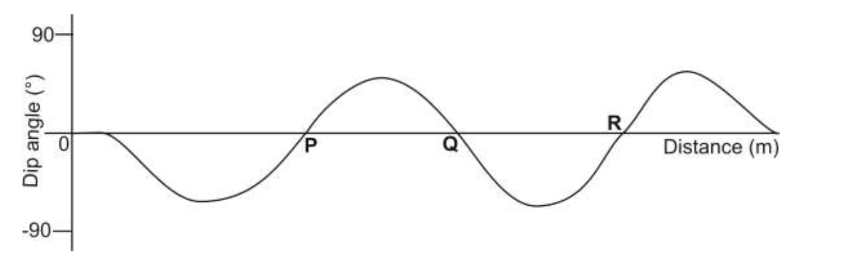
\includegraphics[width=0.5\columnwidth]{figs/10.png}
        \caption*{}
        \label{fig:q10}
    \end{figure}
\begin{multicols}{2}
\begin{enumerate}
\item P, Q and R
\item Q and R
\item P and R
\item P and Q
\end{enumerate}
\end{multicols}

\item The effect of small scale near surface inhomogeneities can be removed from magnetic data by
\hfill(GATE GG 2018)
\begin{enumerate}
\item upward continuation
\item downward continuation
\item second vertical derivative
\item reduction to pole
\end{enumerate}

\item The frequencies of the primary magnetic field generated by worldwide thunderstorm activity vary in the range
\hspace*{15.7cm}(GATE GG 2018)
\begin{multicols}{2}
\begin{enumerate}
\item $10^{-6}$ Hz - $10^{-3}$ Hz
\item $10^{-3}$ Hz - 1 Hz
\item 1 Hz - $10^3$ Hz
\item $10^3$ Hz - $10^6$ Hz
\end{enumerate}
\end{multicols}

\item Assertion \brak{\text{a}}: The Static Self-Potential for a thick, clean freshwater bearing sandstone formation is positive.\\
Reason \brak{\text{r}}: Resistivity of the formation water is less than the resistivity of salt water mud-filtrate.
\hfill(GATE GG 2018)
\begin{enumerate}
\item Both (a) and (r) are true and (r) is the correct reason
\item Both (a) and (r) are true and (r) is not the correct reason
\item Both (a) and (r) are false
\item (a) is true but (r) is false
\end{enumerate}

\item Which one of the following well log responses characterizes an overpressured zone in the subsurface?
\hfill(GATE GG 2018)
\begin{enumerate}
\item High velocity and high resistivity
\item Low velocity and low density
\item High velocity and low resistivity
\item Low velocity and high density
\end{enumerate}

\item The angle of inclination of the remanent magnetization measured on a basalt flow at a location P (28$\degree$N 85$^\degree$E) is 40$\degree$.  
The palaeomagnetic latitude of the basalt flow is \makebox[2cm]{\hrulefill} $\degree$N.
\hfill(GATE GG 2018)
\vspace{0.5cm}

\item Using the Gutenberg-Richter recurrence relationship, the mean annual rate of exceedance of earthquake occurrence in a seismic belt is $0.3$ per year for an earthquake of magnitude $6.0$.  The return period for an earthquake of magnitude $6.0$ in this belt is \makebox[2cm]{\hrulefill} years.
\hfill(GATE GG 2018)
\vspace{0.5cm}

\item In the figure, $Z$ denotes the depth to the center of a buried sphere from the surface and $X_{1/2}$ denotes the half-width of the profile at half the maximum gravity value. The ratio $Z/X_{1/2}$ \makebox[2cm]{\hrulefill} is .
\hfill(GATE GG 2018)
\begin{figure}[H]
        \centering
        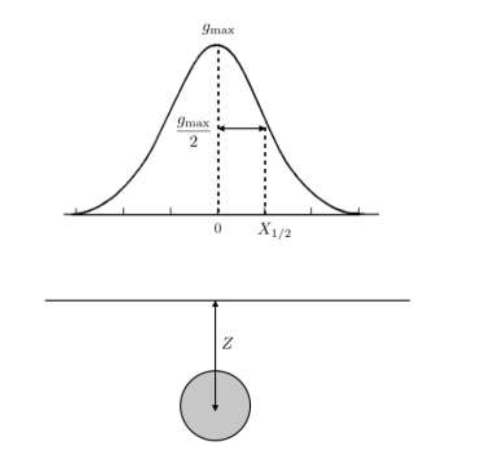
\includegraphics[width=0.5\columnwidth]{figs/11.png}
        \caption*{}
        \label{fig:q10}
    \end{figure}

\item Two survey vessels with shipborne gravimeters are cruising towards each other at $6$ knots each along an E-W course. The difference in gravity readings of the two gravimeters is $63.5$ mGal when they cross. The latitude along which they are cruising is \makebox[2cm]{\hrulefill}$\degree$N.
\hfill(GATE GG 2018)
\vspace{0.5cm}

\item A gravity reading is taken in a stationary helicopter hovering $1$ km above mean sea level at a location. The difference in the value of $g$ measured in the helicopter and at mean sea level beneath it is  \makebox[2cm]{\hrulefill} mGal.
\hfill(GATE GG 2018)
\vspace{0.5cm}

\item The P-wave velocity and Poisson$'$s ratio for a homogeneous isotropic sedimentary rock are $2500$ m/s and $0.3$, respectively. The S-wave velocity for the rock is \makebox[2cm]{\hrulefill} m/s.
\hfill(GATE GG 2018)
\vspace{0.5cm}

\item A plane electromagnetic \brak{\text{EM}} wave travelling vertically downwards with a frequency of $1000$ Hz in a homogeneous medium has a skin depth of $100$ m. The ratio of the amplitude of the EM wave at a depth of $75$ m with respect to the amplitude at the Earth$'$s surface is C.
\hfill(GATE GG 2018)
\vspace{1cm}

\item A student interpreted a four-layer Schlumberger resistivity sounding dataset with resistivities and thicknesses:  
$\rho_1=100\,\Omega m$, $\rho_2=20\,\Omega m$, $\rho_3=1500\,\Omega m$, $\rho_4=50\,\Omega m$, $h_1=50$ m, $h_2=10$ m, $h_3=20$ m. Another student interprets the same data with $\rho_3=2000\,\Omega m$.According to the principle of equivalence, the value of $h_3$ for the second interpretation is \makebox[2cm]{\hrulefill} m.
\hspace*{15.7cm}(GATE GG 2018)
\vspace{0.5cm}

\item The apparent resistivities obtained at $0.1$ Hz and $10$ Hz in a frequency domain I.P. measurement are  $100$ $\Omega$m and $80$ $\Omega$m, respectively.  
The percentage frequency effect is \makebox[2cm]{\hrulefill}.
\hfill(GATE GG 2018)
\vspace{0.5cm}

\item A $15$ V power supply is applied across a cylindrical container \brak{\text{diameter $= 0.20$ m, length $= 0.50$ m}}. Currents measured: $750$ mA \brak{\text{brine only}}, $500$ mA \brak{\text{rock sample fully saturated with brine}}.  The formation factor of the rock sample is \makebox[2cm]{\hrulefill}.
\hspace*{15.7cm}(GATE GG 2018)
\vspace{0.5cm}

\item The ratio of the number of daughter nuclides to parent nuclides after a decay period of $3$ half-lives is \makebox[2cm]{\hrulefill}.
\hspace*{15.7cm}(GATE GG 2018)
\vspace{0.5cm}

\item Consider a laterally homogeneous and isotropic earth model with a flat horizontal surface and three horizontal layers underlain by a half-space. A seismic reflection survey was simulated on this model with the sources and receivers placed on the surface. The table below lists the root mean square (rms) velocities, Vrms, and zero-offset two-way traveltimes to for the three reflection events from the bottom of each of the three layers observed in a pre-stack CDP \brak{\text{CMP}} gather. The interval velocity of the second layer is\makebox[2cm]{\hrulefill} m/s.
\hfill(GATE GG 2018)
\begin{table}[h]
    \centering
    \begin{center}
\begin{tabular}{|c|c|c|}
\hline
\textbf{Reflection Event} & \textbf{$V_{\text{rms}}$ (m/s)} & \textbf{$t_0$ (s)} \\
\hline
1 & 1500m/s & 0.2s \\
\hline
2 & 1600m/s & 0.3s \\
\hline
3 & 1700m/s & 0.4s \\
\hline
\end{tabular}
\end{center}
    \caption{Given Values}
    \label{tab:1}
\end{table}

 \item A spherically symmetric vector field $\vec{g}(r)$ satisfies $\nabla \cdot \vec{g}(r) = -r$. The flux of the vector field through a sphere of unit radius is \makebox[2cm]{\hrulefill} .\brak{\text{Use $\pi=3.14$}}
 \hfill(GATE GG 2018)
 \vspace{0.5cm}

 \item A horizontally travelling surface wave with wavelength $20$ m is attenuated by a linear uniform array of $4$ receivers. The minimum receiver spacing is \makebox[2cm]{\hrulefill}  m.
 \hfill(GATE GG 2018)
 \vspace{0.5cm}
 
\item An end-on marine survey is carried out with equal shot and receiver spacing.If the total number of shots fired is $50$ and the total number of traces recorded is $10000$, the maximum fold of the survey is \makebox[2cm]{\hrulefill}
\hfill(GATE GG 2018)
\vspace{0.5cm}

\item The highest singular value of the matrix $G=\begin{pmatrix} 1 & 2 &1 \\ -1 & 2 & 0 \end{pmatrix}$ is \makebox[2cm]{\hrulefill}.
\hfill(GATE GG 2018)\\

\textbf{END OF THE QUESTION PAPER}
    \end{enumerate}
\end{document}
